\documentclass[17pt]{beamer} %Makes presentation
%\documentclass[14pt, handout]{beamer} %Makes Handouts

%\usetheme{Singapore} %Gray with fade at top
%\useoutertheme[subsection=false]{miniframes} %Supppress subsection in header
%\useinnertheme{rectangles} %Itemize/Enumerate boxes
%\usecolortheme{seagull} %Color theme
%\usecolortheme{rose} %Inner color theme

% white on black
\setbeamercolor{normal text}{fg=white,bg=blue!20!black}
\setbeamercolor{structure}{fg=white, bg=blue!20!black}
\setbeamercolor{alerted text}{fg=yellow!70!orange}
%\setbeamercolor{item projected}{use=item,fg=black,bg=item.fg!35}
\setbeamercolor*{palette primary}{use=structure,fg=structure.fg}
\setbeamercolor*{palette secondary}{use=structure,fg=structure.fg!95!black}
\setbeamercolor*{palette tertiary}{use=structure,fg=structure.fg!90!black}
\setbeamercolor*{palette quaternary}{use=structure,fg=structure.fg!95!black,bg=black!80}
\setbeamercolor*{framesubtitle}{fg=white}
\setbeamercolor*{block title}{use=structure, bg=blue!20!black}
\setbeamercolor*{block body}{use=structure}


\definecolor{light-gray}{gray}{0.75}
\definecolor{dark-gray}{gray}{0.55}
\setbeamercolor{item}{fg=light-gray}
\setbeamercolor{enumerate item}{fg=dark-gray}

\setbeamertemplate{navigation symbols}{}
%\setbeamertemplate{mini frames}[default]
%\setbeamercovered{dynamics}
\setbeamerfont*{title}{size=\Large,series=\bfseries}

%\setbeameroption{notes on second screen} %Dual-Screen Notes
%\setbeameroption{show only notes} %Notes Output

\setbeamertemplate{frametitle}{\vspace{.5em}\bfseries\insertframetitle}
\newcommand{\heading}[1]{\noindent \textbf{#1}\\ \vspace{1em}}

% small footnotes
\setbeamerfont{footnote}{size=\tiny}

\usepackage{bbding,color,multirow,times,ccaption,tabularx,graphicx,verbatim,booktabs,fixltx2e}
\usepackage{colortbl} %Table overlays
\usepackage[english]{babel}
\usepackage[latin1]{inputenc}
\usepackage[T1]{fontenc}
\usepackage{lmodern}
\usepackage{alltt}
\usepackage{textcomp} % copyright/trademark
\usepackage{animate}

\usepackage{tikz}
\usetikzlibrary{positioning}
\usetikzlibrary{trees}


% black slide
\newcommand{\bigslide}[1]{
\bgroup
\setbeamercolor{background canvas}{bg=black}
\begin{frame}[plain]{}

\Huge
\begin{center}
\textbf{\textcolor{white}{#1}}
\end{center}
\end{frame}
\egroup
}




\author[]{Thomas J. Leeper}
\institute[]{
  \inst{}%
  Department of Government\\London School of Economics and Political Science
}

\title{{\Large Treadmills\\Fractals\\Apples and Oranges}}

\date[]{11 November 2017}

\begin{document}

\frame{\titlepage}


\section{Treadmills}

\bigslide{Treadmills}

\frame{
\centering

\includegraphics[height=\textheight]{images/treadmill.png}
}


\frame{

\frametitle{Treadmills}

\begin{itemize}\itemsep1em
\item Science is supposed to be about climbing a ladder of hidden knowledge to uncover truth
\item<2-> The science of media exposure is more of a treadmill or a Stairmaster\textsuperscript{\textregistered}
\end{itemize}

}


\frame{

\frametitle{{\normalsize Brief History of Measurement}}

\begin{itemize}\itemsep1em
\item Binary
	\begin{itemize}
	\item The simplest and earliest measures of media exposure were binary
	\end{itemize}
\item Ordinal 
	\begin{itemize}
	\item \dots rankings of sources/outlets
	\item \dots self-reported degree of attentiveness
	\end{itemize}
\item Interval
	\begin{itemize}
	\item Time-based, frequency-based, and passive measures
	\end{itemize}
\end{itemize}

}


\frame<1-2>[label=solutions]{

\frametitle{Solutions?}

\begin{itemize}\itemsep1em
\item<2-> More specific measures
\item<3-> ``Program List'' method
\item<4-> Passive (radio, tv, web) tracking
\item<5-> Some as-of-yet-undiscovered method
\end{itemize}

\only<6->{Measures and our ability to validate them are time and context dependent!}
% thus we never get anywhere
}

\frame{

\frametitle{History and Measures}

\footnotesize
\centering 
\begin{tabular}{lc}
\textbf{Program} & \textbf{Years Measured by Pew BMCS} \\ \midrule
``Evening News'' & 1996--2012 \\
``Local TV'' & 1996--2012 \\
``Local cable'' & 2000 \\
MTV & 1996--1998 \\
Limbaugh & 1996--98, 2002--2012 \\
A Current Affair & 1996--1998, 2008 \\
Daytime talk shows & 1996--2002, 2012 \\
Court TV & 1998--2000 \\
Today Show & 1998--2004, 2008--2012 \\
Keith Olbermann & 2008--2010 \\
Daily Show & 2002--2012 \\
Glenn Beck & 2010 \\
\dots 
\end{tabular}
}

\againframe<2->{solutions}




\section{Fractals}

\bigslide{Fractals}

\frame{

How long is the coastline of Britain?

\onslide<2->{

\begin{center}
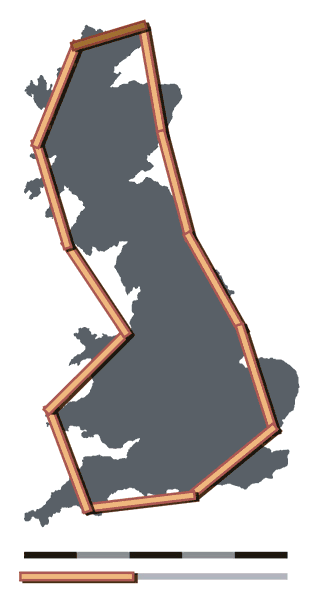
\includegraphics[width=.25\textwidth]{images/Britain-fractal-coastline-200km.png}%
\hspace{0.5em}
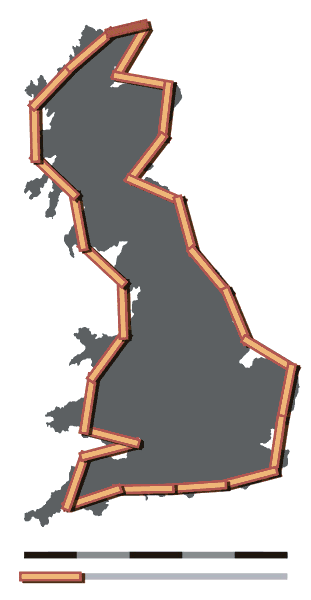
\includegraphics[width=.25\textwidth]{images/Britain-fractal-coastline-100km.png}%
\hspace{0.5em}
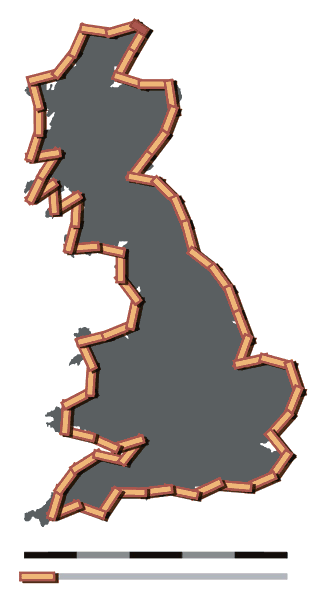
\includegraphics[width=.25\textwidth]{images/Britain-fractal-coastline-50km.png}%
\end{center}

It depends on the length of your ruler.
}

}

\frame{

How much media exposure has a given person experienced?

\vspace{2em}

\onslide<2->{It depends on the precision and form of your measure.}

}


\frame{

\frametitle{{\normalsize The treadmill reveals fractals}}

\begin{itemize}\itemsep1em
\item Source-based measures reveal the landscape is infinitely diverse
	\begin{itemize}
	\item We are far removed from the 1950s (US) or dominant public broadcaster (Europe) media landscape
	\item What is the population of media content?
	\end{itemize}

\item<2-> Our measures are never fully informative
	\begin{itemize}
	\item Hours in a day
	\item Stories in a week
	\item \dots
	\end{itemize}
\end{itemize}

}

\frame{

\frametitle{Source--Frequency Nexus}

If the number of sources is infinite and the right metric of media time-use is possibly and meaningfully infinitely small, we cannot conceptualize the totality of an individual's exposure to media let alone measure it using any self-report or passive device.

}

\frame{

And that doesn't even begin to address:

\begin{itemize}
\item Secondhand exposure
\item News links or content on social media
\item Dual screening
\item Active/passive distinctions
\item Exposure/attention/reception
\end{itemize}
}


\section{Apples and Oranges}

\bigslide{Apples\\ and\\ Oranges}

\frame{
\vspace{0.5em}
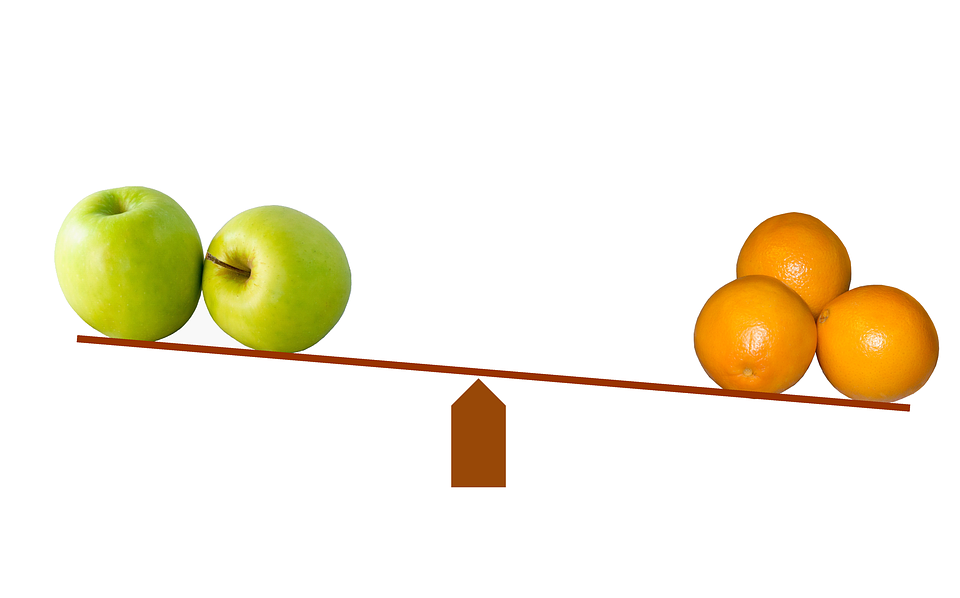
\includegraphics[width=\textwidth]{images/apples-and-oranges.png}
}

\frame{

\frametitle{Apples and Oranges}

\small

\begin{itemize}
\item<2-> Is a minute of New York Times equivalent to a minute of Wall Street Journal?
\item<3-> Is a minute of television equivalent to a minute of radio?
\item<4-> Is a minute of CNN equivalent to a minute of Bret Stephens?
\item<5-> Is a minute of Reddit equivalent to a minute of DR1?
\item<6-> Is a minute of 1960s CBS equivalent to a minute of Twitter?
\end{itemize}

}

\frame{

\frametitle{Apples and Oranges}

\begin{itemize}
\item<2-> Is the effect of the New York Times the same for everyone and at all times?
\item<3-> Is the effect of television the same for everyone and at all times?
\item<4-> Is the effect of Facebook the same for everyone and at all times?
\end{itemize}

}

\frame{

\frametitle{Apples and Oranges}

If we can't even compare `like with like'

\begin{itemize}
\item New York Times and Wall Street Journal
\item CNN in 1998 and CNN in 2017
\item Facebook for you and Facebook for me
\end{itemize}

\onslide<2->{how can we meaningfully study the effects of exposure across media, across time, across geography, and across people?}

}



\frame{

\frametitle{Content, topics, \& events}

\large

If time-use and source-based metrics are fundamentally flawed, what can we do instead?

\vspace{1em}

One answer is to focus on \textbf{content}.

}

\frame{

\frametitle{Content, topics, \& events}

But what are relevant aspects of content?

\begin{itemize}
\item Broad topic
\item Specific facts
\item Tone
\item Frame
\item Ideology
\item \dots
\end{itemize}
}


\bigslide{So what?}

\frame{

\frametitle{Three huge problems}

\begin{enumerate}\itemsep1em
\item Treadmills
\item Fractals
\item Apples and oranges
\end{enumerate}

}

\frame{

\frametitle{Three huge problems}

\begin{enumerate}\itemsep1em
\item You can't reach the end of the treadmill, even if you run really fast!
\item Are \textbf{time-use} and \textbf{source} even the right ways to be theorizing media?
\item Media and exposure experiences are not comparable, we just pretend they are.
\end{enumerate}

}



\frame{

%\frametitle{{\normalsize Where do we go from here?}}

We need to get off the treadmill.

}


\frame{

\frametitle{{\normalsize Where do we go from here?}}

\large 

\begin{enumerate}\itemsep1em
\item<2-> Thick description
\item<3-> Forward causal inference
\item<4-> Effect heterogeneity
\item<5-> Research design
\end{enumerate}

}


\frame{

Experiments are never going to be able to comprehensively and generalizably describe the effects of media.

\vspace{1em}

\onslide<2->{But that's an unobtainable ideal\onslide<3->{, so we should do the best we can.}}

}


\bigslide{}

\end{document}
